\savestack{\nn}{% \hspace{-0.1in}
\tikzstyle{input_neuron}=[circle,draw=red!50,fill=red!10,thick,minimum size=8mm]
\tikzstyle{hidden_neuron}=[circle,draw=blue!50,fill=cyan!10,thick,minimum size=8mm]
\tikzstyle{output_neuron}=[circle,draw=green!50,fill=green!10,thick,minimum size=8mm]
\tikzstyle{bias_neuron}=[circle,draw=red!50,fill=red!10,thick,minimum size=4mm]
\tikzstyle{bias_hidden_neuron}=[circle,draw=blue!50,fill=cyan!10,thick,minimum size=4mm]
\tikzstyle{input}=[circle,draw=black!50,fill=black!20,thick,minimum size=8mm]
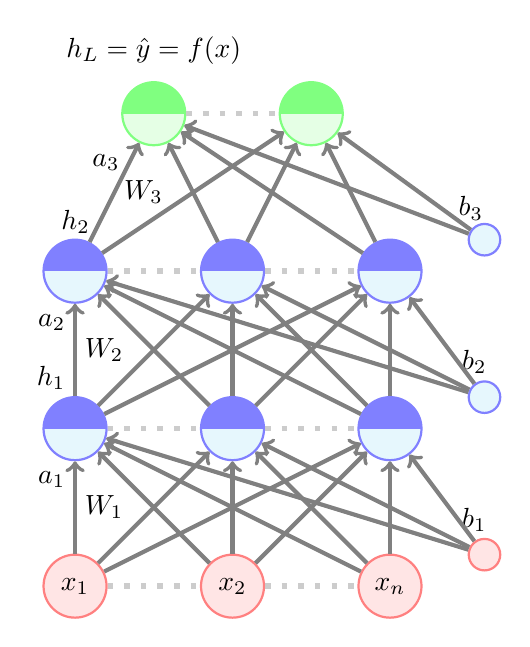
\begin{tikzpicture}
	\node [input_neuron] (neuron01) at (0,0) {$x_1$};
	\node [input_neuron] (neuron02) at (2,0){$x_2$};
	\node [input_neuron] (neuron03) at (4,0) {$x_n$};

	\node [bias_neuron] (neuron04) at (5.2,0.4) {};

	\node [hidden_neuron] (neuron11) at (0,2)  {};
	\node [hidden_neuron] (neuron12) at (2,2)  {};
	\node [hidden_neuron] (neuron13) at (4,2)  {};

	\node [bias_hidden_neuron] (neuron14) at (5.2,2.4) {};

	\begin{scope}
		\path[clip] (0,2) circle (4mm);
		\path[fill=blue!50] (-0.4,2) rectangle (0.4,2.4);
	\end{scope}

	\begin{scope}
		\path[clip] (2,2) circle (4mm);
		\path[fill=blue!50] (1.6,2) rectangle (2.4,2.4);
	\end{scope}

	\begin{scope}
		\path[clip] (4,2) circle (4mm);
		\path[fill=blue!50] (3.6,2) rectangle (4.4,2.4);
	\end{scope}

	\node [hidden_neuron] (neuron21) at (0,4)  {};
	\node [hidden_neuron] (neuron22) at (2,4)  {};
	\node [hidden_neuron] (neuron23) at (4,4)  {};

	\node [bias_hidden_neuron] (neuron24) at (5.2,4.4) {};

	\begin{scope}
		\path[clip] (0,4) circle (4mm);
		\path[fill=blue!50] (-0.4,4) rectangle (0.4,4.4);
	\end{scope}

	\begin{scope}
		\path[clip] (2,4) circle (4mm);
		\path[fill=blue!50] (1.6,4) rectangle (2.4,4.4);
	\end{scope}
	\begin{scope}
		\path[clip] (4,4) circle (4mm);
		\path[fill=blue!50] (3.6,4) rectangle (4.4,4.4);
	\end{scope}

	\node [output_neuron] (neuron31) at (1,6)  {};
	\node [output_neuron] (neuron32) at (3,6)  {};

	\begin{scope}
		\path[clip] (1,6) circle (4mm);
		\path[fill=green!50] (0.6,6) rectangle (1.4,6.4);
	\end{scope}

	\begin{scope}
		\path[clip] (3,6) circle (4mm);
		\path[fill=green!50] (2.6,6) rectangle (3.4,6.4);
	\end{scope}

	\draw[white,->] (neuron01) -- (neuron11) node[black,pos=.5,right]  {$W_{1}$} node[black,pos=0.8,left] {$a_{1}$};

	\draw[white,->] (neuron11) -- (neuron21) node[black,pos=.5,right] {$W_{2}$} node[black,pos=0.8,left] {$a_{2}$} node[black,pos=.2,left] {$h_{1}$};
	\draw[white,->] (neuron21) -- (neuron31) node[black,pos=.5,right] {$W_{3}$} node[black,pos=0.8,left] {$a_{3}$} node[black,pos=.2,left] {$h_{2}$};
	\draw[white,->] (neuron04) -- (neuron13) node[black,pos=0,right,above] {$b_1$};
	\draw[white,->] (neuron14) -- (neuron23) node[black,pos=0,right,above] {$b_2$};
	\draw[white,->] (neuron24) -- (neuron32) node[black,pos=0,right,above] {$b_3$};

	\draw[white,->] (neuron31) -- (1,6.5) node[black,pos=1,above] {$h_L = \hat{y} = f(x)$};

	\draw[black!20,line width=2pt,loosely dotted] (neuron01) -- (neuron02);
	\draw[black!20,line width=2pt,loosely dotted] (neuron02) -- (neuron03);
	\draw[black!20,line width=2pt,loosely dotted] (neuron11) -- (neuron12);
	\draw[black!20,line width=2pt,loosely dotted] (neuron12) -- (neuron13);
	\draw[black!20,line width=2pt,loosely dotted] (neuron21) -- (neuron22);
	\draw[black!20,line width=2pt,loosely dotted] (neuron22) -- (neuron23);
	\draw[black!20,line width=2pt,loosely dotted] (neuron31) -- (neuron32);

	\foreach \from in {neuron01,neuron02,neuron03,neuron04}
	\foreach \to in {neuron11,neuron12,neuron13}
	\draw [black!50,line width=1.5pt,->] (\from) -- (\to);

	\foreach \from in {neuron11,neuron12,neuron13,neuron14}
	\foreach \to in {neuron21,neuron22,neuron23}
	\draw [black!50,line width=1.5pt,->] (\from) -- (\to);

	\foreach \from in {neuron21,neuron22,neuron23,neuron24}
	\foreach \to in {neuron31,neuron32}
	\draw [black!50,line width=1.5pt,->] (\from) -- (\to);
\end{tikzpicture}}

\begin{frame}
  \myheading{Module 4.1: Feedforward Neural Networks (a.k.a. multilayered network of neurons)}
\end{frame}

%Slide 04
\begin{frame}
  \begin{columns}
    \column{0.35\textwidth}
    \begin{overlayarea}{\textwidth}{\textheight}
      \hspace{-0.1in}
\tikzstyle{input_neuron}=[circle,draw=red!50,fill=red!10,thick,minimum size=8mm]
\tikzstyle{hidden_neuron}=[circle,draw=blue!50,fill=cyan!10,thick,minimum size=8mm]
\tikzstyle{output_neuron}=[circle,draw=green!50,fill=green!10,thick,minimum size=8mm]
\tikzstyle{bias_neuron}=[circle,draw=red!50,fill=red!10,thick,minimum size=4mm]
\tikzstyle{bias_hidden_neuron}=[circle,draw=blue!50,fill=cyan!10,thick,minimum size=4mm]

\tikzstyle{input}=[circle,draw=black!50,fill=black!20,thick,minimum size=8mm]

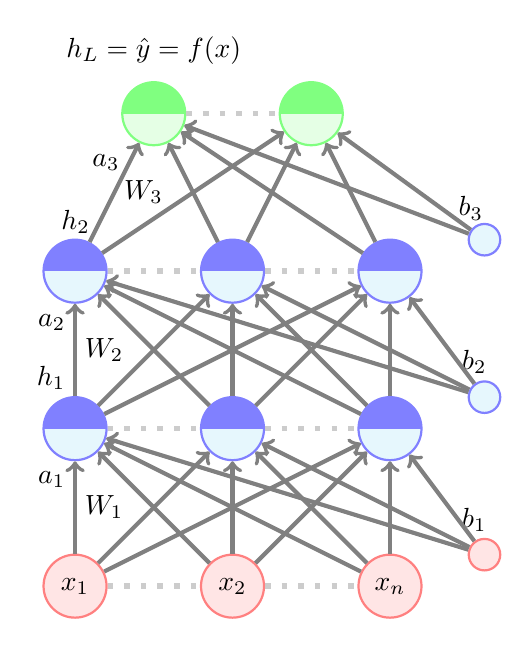
\begin{tikzpicture}
	\onslide<2->{\node [input_neuron] (neuron01) at (0,0) {$x_1$};}
	\onslide<2->{\node [input_neuron] (neuron02) at (2,0) {$x_2$};}
	\onslide<2->{\node [input_neuron] (neuron03) at (4,0) {$x_n$};}

	\onslide<13->{\node [bias_neuron] (neuron04) at (5.2,0.4) {};}


	\onslide<4->{\node [hidden_neuron] (neuron11) at (0,2)  {};}
	\onslide<4->{\node [hidden_neuron] (neuron12) at (2,2)  {};}
	\onslide<4->{\node [hidden_neuron] (neuron13) at (4,2)  {};}

	\onslide<14->{\node [bias_hidden_neuron] (neuron14) at (5.2,2.4) {};}

	\onslide<8->{
		\begin{scope}
			\path[clip] (0,2) circle (4mm);
			\path[fill=blue!50] (-0.4,2) rectangle (0.4,2.4);
		\end{scope}
		\begin{scope}
			\path[clip] (2,2) circle (4mm);
			\path[fill=blue!50] (1.6,2) rectangle (2.4,2.4);
		\end{scope}
		\begin{scope}
			\path[clip] (4,2) circle (4mm);
			\path[fill=blue!50] (3.6,2) rectangle (4.4,2.4);
		\end{scope}
	}

	\onslide<4->{\node [hidden_neuron] (neuron21) at (0,4)  {};}
	\onslide<4->{\node [hidden_neuron] (neuron22) at (2,4)  {};}
	\onslide<4->{\node [hidden_neuron] (neuron23) at (4,4)  {};}

	\onslide<15->{\node [bias_hidden_neuron] (neuron24) at (5.2,4.4) {};}

	\onslide<8->{
		\begin{scope}
			\path[clip] (0,4) circle (4mm);
			\path[fill=blue!50] (-0.4,4) rectangle (0.4,4.4);
		\end{scope}
		\begin{scope}
			\path[clip] (2,4) circle (4mm);
			\path[fill=blue!50] (1.6,4) rectangle (2.4,4.4);
		\end{scope}
		\begin{scope}
			\path[clip] (4,4) circle (4mm);
			\path[fill=blue!50] (3.6,4) rectangle (4.4,4.4);
		\end{scope}
	}

	\onslide<6->{
		\node [output_neuron] (neuron31) at (1,6)  {};
		\node [output_neuron] (neuron32) at (3,6)  {};
	}

	\onslide<8->{
		\begin{scope}
			\path[clip] (1,6) circle (4mm);
			\path[fill=green!50] (0.6,6) rectangle (1.4,6.4);
		\end{scope}
		\begin{scope}
			\path[clip] (3,6) circle (4mm);
			\path[fill=green!50] (2.6,6) rectangle (3.4,6.4);
		\end{scope}
	}

	\onslide<9->{\draw[white,->] (neuron01) -- (neuron11) node[black,pos=0.8,left] {$a_{1}$} ;}
	\onslide<9->{\draw[white,->] (neuron11) -- (neuron21) node[black,pos=0.8,left] {$a_{2}$} ;}
	\onslide<9->{\draw[white,->] (neuron21) -- (neuron31) node[black,pos=0.8,left] {$a_{3}$} ;}

	\onslide<10->{\draw[white,->] (neuron11) -- (neuron21) node[black,pos=.2,left] {$h_{1}$};}
	\onslide<10->{\draw[white,->] (neuron21) -- (neuron31) node[black,pos=.2,left] {$h_{2}$};}
	\onslide<10->{\draw[white,->] (neuron31) -- (1,6.5) node[black,pos=1,above] {$h_L = \hat{y} = f(x)$};}


	\onslide<13->{\draw[white,->] (neuron01) -- (neuron11) node[black,pos=.5,right]  {$W_{1}$} ;}
	\onslide<13->{\draw[white,->] (neuron04) -- (neuron13) node[black,pos=0,right,above] {$b_1$};}

	\onslide<14->{\draw[white,->] (neuron11) -- (neuron21) node[black,pos=.5,right] {$W_{2}$} ;}
	\onslide<14->{\draw[white,->] (neuron14) -- (neuron23) node[black,pos=0,right,above] {$b_2$};}

	\onslide<15->{\draw[white,->] (neuron21) -- (neuron31) node[black,pos=.5,right] {$W_{3}$} ;}
	\onslide<15->{\draw[white,->] (neuron24) -- (neuron32) node[black,pos=0,right,above] {$b_3$};}



	%\draw[white,->] (neuron31) -- (3,6.5) node[black,pos=1,above] {$f(x)$};
	%node[pos=1.3,above,right] {$\mathscr{L}(\theta)$};

	\onslide<2->{\draw[black!20,line width=2pt,loosely dotted] (neuron01) -- (neuron02);
		\draw[black!20,line width=2pt,loosely dotted] (neuron02) -- (neuron03);}

	\onslide<4->{\draw[black!20,line width=2pt,loosely dotted] (neuron11) -- (neuron12);
		\draw[black!20,line width=2pt,loosely dotted] (neuron12) -- (neuron13);}

	\onslide<4->{\draw[black!20,line width=2pt,loosely dotted] (neuron21) -- (neuron22);
		\draw[black!20,line width=2pt,loosely dotted] (neuron22) -- (neuron23);}

	\onslide<6->{\draw[black!20,line width=2pt,loosely dotted] (neuron31) -- (neuron32);}

	\onslide<13->{
		\foreach \from in {neuron01,neuron02,neuron03,neuron04}
		\foreach \to in {neuron11,neuron12,neuron13}
		\draw [black!50,line width=1.5pt,->] (\from) -- (\to);
	}

	\onslide<14->{
		\foreach \from in {neuron11,neuron12,neuron13,neuron14}
		\foreach \to in {neuron21,neuron22,neuron23}
		\draw [black!50,line width=1.5pt,->] (\from) -- (\to);
	}

	\onslide<15->{
		\foreach \from in {neuron21,neuron22,neuron23,neuron24}
		\foreach \to in {neuron31,neuron32}
		\draw [black!50,line width=1.5pt,->] (\from) -- (\to);
	}

\end{tikzpicture}


    \end{overlayarea}

    \column{0.65\textwidth}
    \begin{overlayarea}{\textwidth}{\textheight}
      \begin{itemize}
        % \justifying
        \item<1-> The input to the network is an $\mathbf{n}$-dimensional vector
        \item<3-> The network contains $\mathbf{L-1}$ hidden layers (2, in this case) having $\mathbf{n}$ neurons each
        \item<5-> Finally, there is one output layer containing $\mathbf{k}$ neurons (say, corresponding to $\mathbf{k}$ classes)
        \item<7-> Each neuron in the hidden layer and output layer can be split into two parts : \visible<9->{pre-activation} \visible<10->{and activation} \visible<11->{($a_i$ and $h_i$ are vectors)}
        \item<12-> The input layer can be called the $0$-th layer and the output layer can be called the $(L)$-th layer
        \item<13-> $W_i \in \mathbb{R}^{n\times n}$ and $b_i \in \mathbb{R}^n$ are the weight and bias between layers $i-1$ and $i$  ($0<i<L$)
        \item<15-> $W_{L} \in \mathbb{R}^{n\times k}$ and $b_{L} \in \mathbb{R}^k$ are the weight and bias between the last hidden layer and the output layer ($L = 3$ in this case)
      \end{itemize}
    \end{overlayarea}
  \end{columns}
\end{frame}

%Slide 05
\begin{frame}
  \begin{columns}
    \column{0.35\textwidth}
    \begin{overlayarea}{\textwidth}{\textheight}
      \makebox[\textwidth][c]{\usebox{\nncontent}}
    \end{overlayarea}

    \column{0.65\textwidth}
    \begin{overlayarea}{\textwidth}{\textheight}
      \begin{itemize}
        % \justifying
        \item<1-> The pre-activation at layer $i$ is given by
          \begin{align*}
            a_i(x) = b_i + W_i h_{i-1}(x)
          \end{align*}
        \item<2-> The activation at layer $i$ is given by
          \begin{align*}
            h_i(x) = g(a_i(x))
          \end{align*}

          \visible<3->{
              \noindent where $g$ is called the activation function (for example, logistic, tanh, linear, \textit{etc.})
          }
        \item<4-> The output at layer $i$ is given by
            \begin{align*}
              f(x) = h_{L+1}(x) = O(a_{L+1}(x))
            \end{align*}
            \visible<5->{
              \noindent where $O$ is the output activation function (for example, softmax, linear, \textit{etc.})
            }
        \item<6-> To simplify notation we will refer to $a_i(x)$ as $a_i$ and $h_i(x)$ as $h_i$
      \end{itemize}
    \end{overlayarea}
  \end{columns}
\end{frame}

%Slide 06
\begin{frame}
  \begin{columns}
    \column{0.35\textwidth}
    \begin{overlayarea}{\textwidth}{\textheight}
      \makebox[\textwidth][c]{\usebox{\nncontent}}
    \end{overlayarea}

    \column{0.65\textwidth}
    \begin{overlayarea}{\textwidth}{\textheight}
      \begin{itemize}
        % \justifying
        \item The pre-activation at layer $i$ is given by
            \begin{align*}
              a_i = b_i + W_i h_{i-1}
            \end{align*}
        \item The activation at layer $i$ is given by
            \begin{align*}
              h_i = g(a_i)
            \end{align*}
            where $g$ is called the activation function (for example, logistic, tanh, linear, \textit{etc.})
        \item The activation at layer $i$ is given by
            \begin{align*}
              f(x) = h_{L+1} = O(a_{L+1})
            \end{align*}
            where $O$ is the output activation function (for example, softmax, linear, \textit{etc.})
      \end{itemize}
    \end{overlayarea}

  \end{columns}
\end{frame}

%Slide 07
\begin{frame}
  \begin{columns}
    \column{0.35\textwidth}
    \begin{overlayarea}{\textwidth}{\textheight}
      \makebox[\textwidth][c]{\usebox{\nncontent}}
    \end{overlayarea}

    \column{0.65\textwidth}
    \visible <1-5> {
      \begin{itemize}
        % \justifying
        \item <1-> \textbf{Data:} $\left\{ x_{i},y_{i} \right\}_{i=1}^{N}$
        \item <2->  \textbf{Model:} \begin{align*}\hat y_{i} = f(x_{i}) = O(W^{3}g(W^{2}g(W^{1}x+b_{1})+b_{2})+b_{3})\end{align*}
        \item <3-> \textbf{Parameters:} $\quad \theta = {W_{1}, .., W_{L}, b_1, b_2, ... , b_L} (L =3)$
        \item <4-> \textbf{Algorithm:} Backpropagation
        \item <5-> \textbf{Objective/Loss/Error function:} Say,
            \vspace{-0.2in}
            \begin{align*}
              min                        & ~ \frac{1}{N} \sum_{i=1}^{N} (\hat y_{i} - y_{i})^{2} \\
              \textit{In general,} ~ min & ~ \mathscr{L}(\theta)
            \end{align*}
            where $\mathscr{L}(\theta)$ is some function of the parameters
      \end{itemize}
    }
  \end{columns}
\end{frame}
